\section{Results}

Our experiment measured the eye and body movements as participants performed a sorting task in a virtual environment. The participants sorted objects based on the color and/or shape where we modulated the task complexity into EASY and HARD trials. We further divided the trials into planning and execution epochs where participants planned the selection of the target objects to grasp and then executing the action of displacing it to target shelves, respectively. In this section, we report the behavioral and oculomotor differences of the subjects for the two task types (EASY, HARD), and the planning and execution epochs.

\subsection{Task based Behavioral Differences}
In the present study, the primary object related action was to repeatedly pickup objects and place them at a desired locations until they were sorted according to the sorting task. To account for the behavioral differences between the task complexities, we used the measure of trial duration and the number of object displacements required to completet the tasks. \textcolor{Blue}{Figure \ref{figure:easy_hard_diff}A} shows the differences in EASY and HARD trials based on the time taken to finish the sorting task. A two-sample independent t-test showed that the trial duration for the two trial types were significantly different ($t = -10.13, p < 0.001$) where EASY trials that required the objects to be sorted based on a single feature were  shorter ($Mean = 54.12 seconds, SD = 13.33$) as compared to HARD trials ($Mean = 111.57 seconds, SD = 36.92$) where subjects had to sort taking into account both features (color and shape) of the objects. 

\textcolor{Blue}{Figure \ref{figure:easy_hard_diff}B} shows the comparisons in the object displacements made by the subjects and the optimal number of displacements as elicited by the optimal model for both EASY and HARD trials. Subjects made lower number of object displacements in the EASY trials ($ Mean = 10.2, SD = 1.99$) compared to HARD trials ($Mean = 15.52, SD = 2.59$). In the EASY trials the model required lower number of object displacements ($Mean = 9.42, SD = 1.48$) displacements, whereas, in the HARD trials, model required higher number of displacements ($Mean = 11.24, SD = 2.77$). We compared the human and model performance for the two trial types using independent t-tests. In the EASY trials, there was a significant difference between the model and human object displacements ($t=3.64, p<0.001$). In the HARD trials, there was also a significant difference between the model and human performance ($t=10,61, p<0.001$). This indicates that the participants did not plan their actions optimally and might have used other heuristics to complete the task.

\begin{figure}[ht]
    \centering
    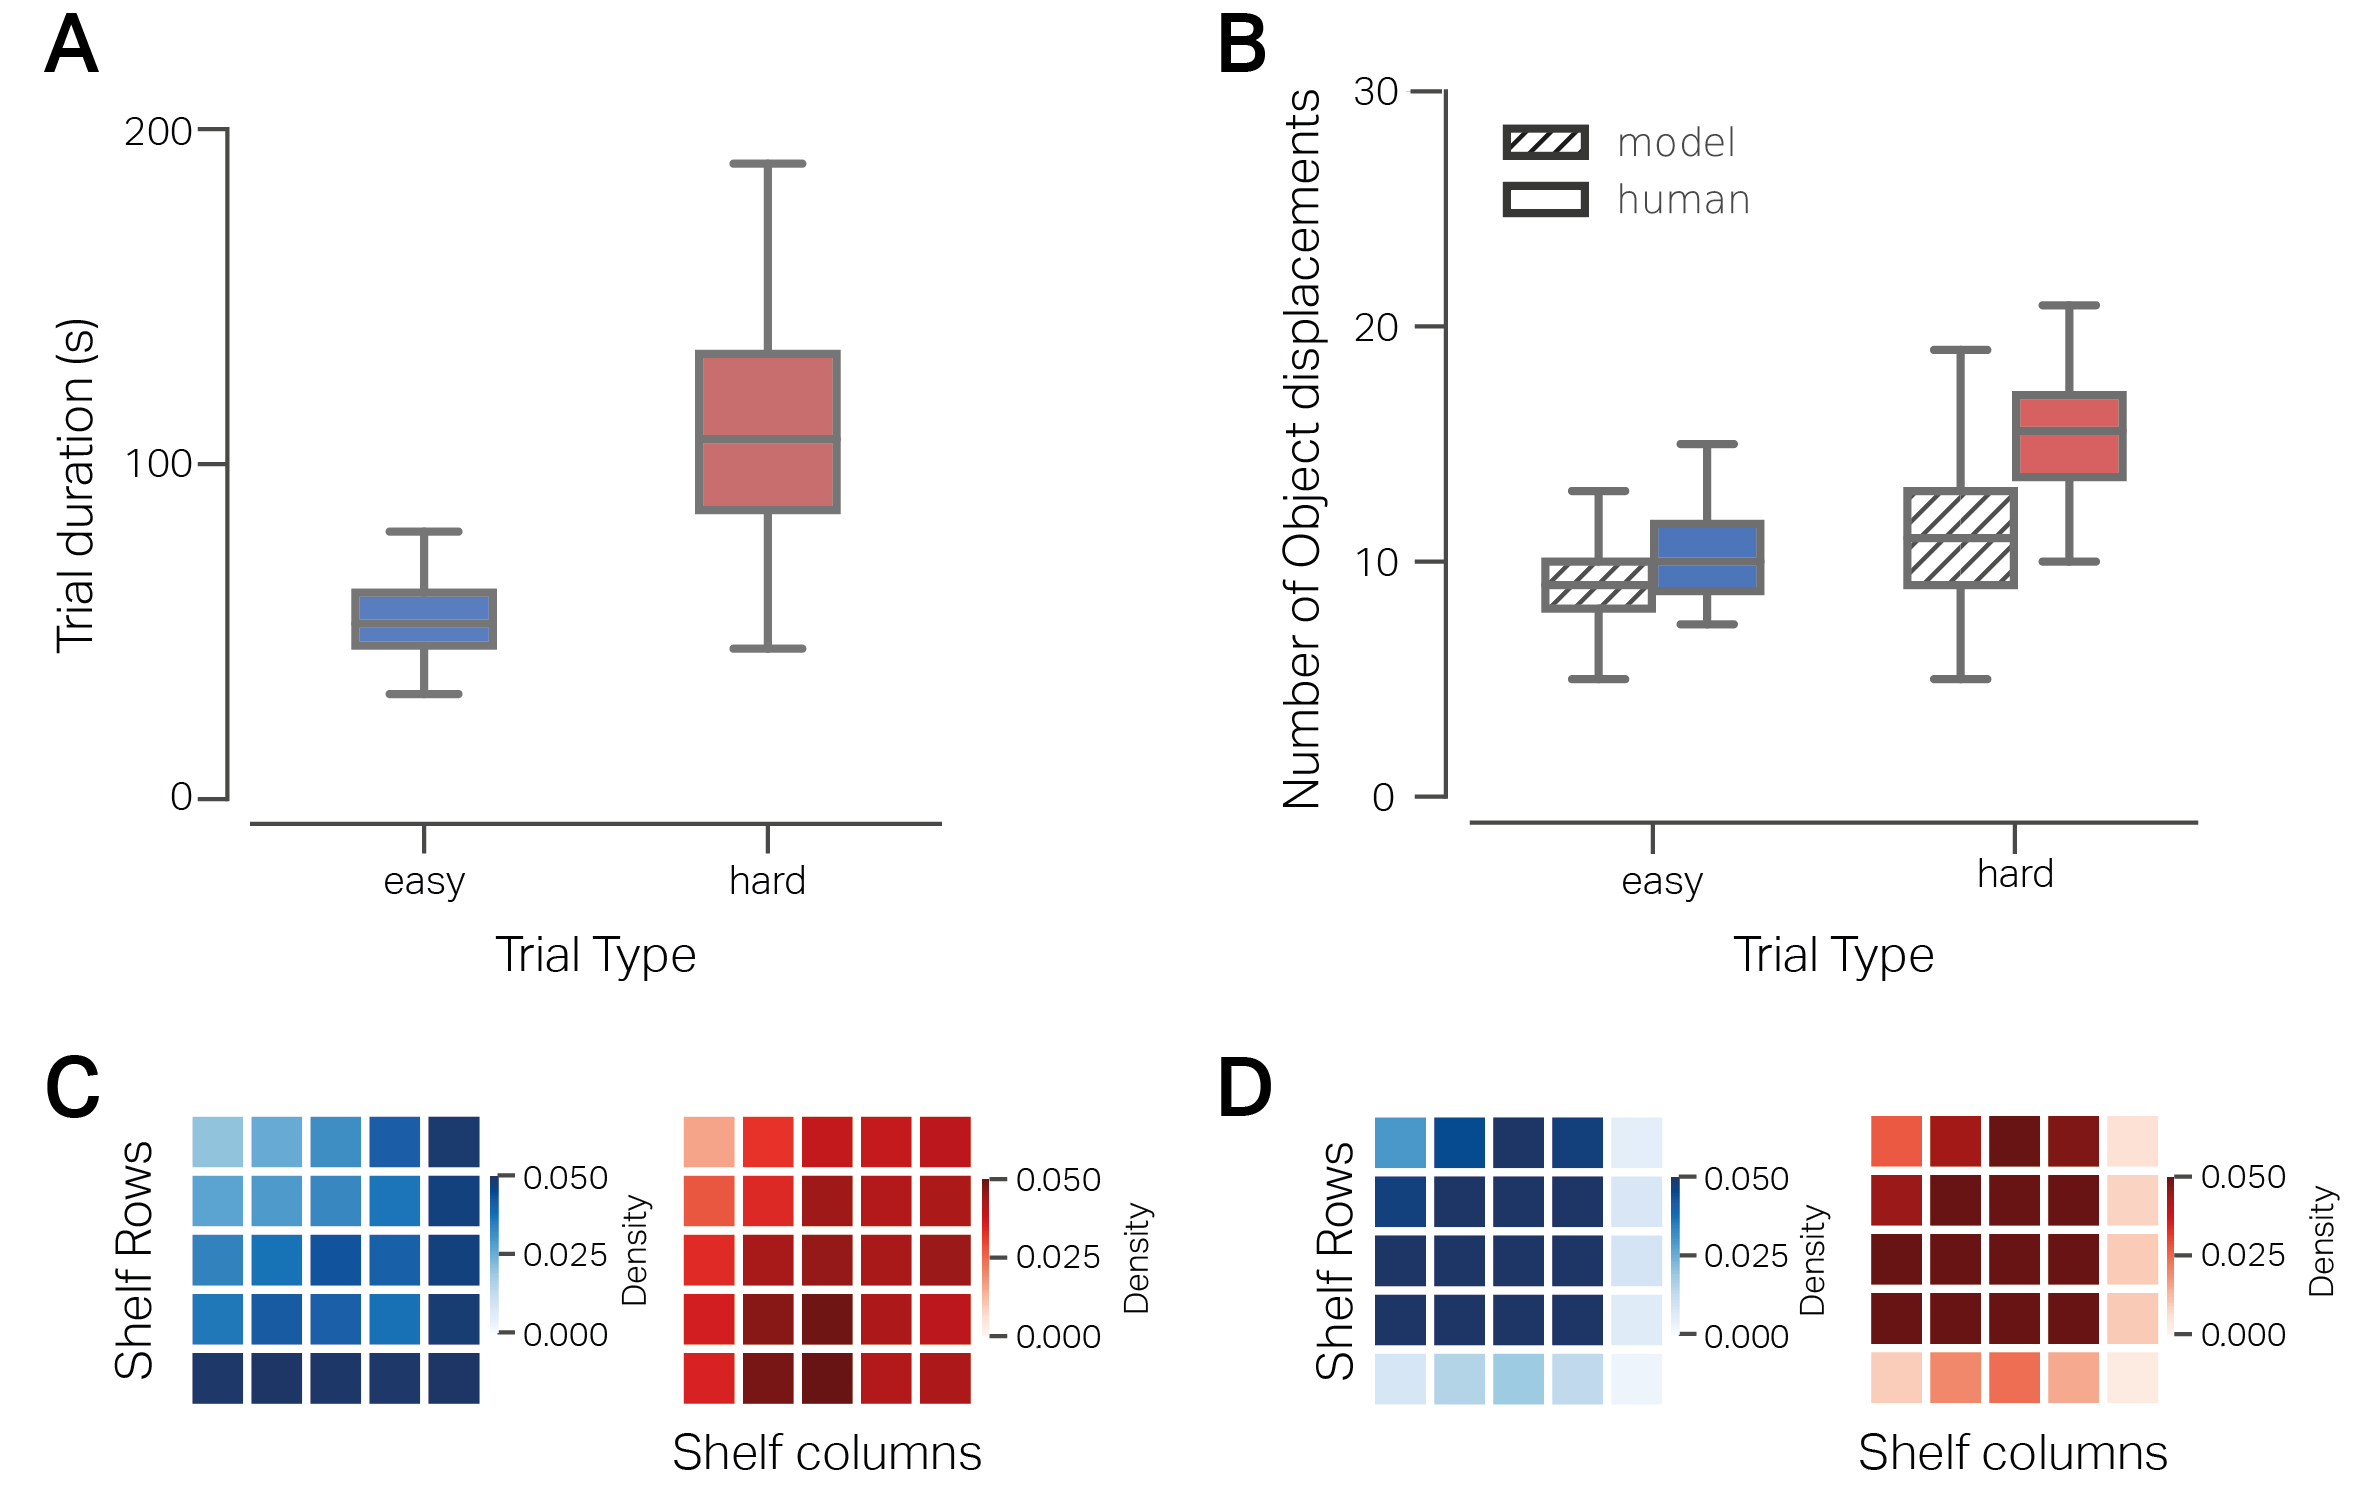
\includegraphics[width=1\linewidth]{source/figures/results/results_1.png} 
    \caption[Behavioral differences based on the 2 tasks]{\textbf{A.} Trial duration of the EASY and HARD trials. The boxplots show the inter-quartile range (IQR) of the duration of the trials for the two different trial types for all trials and participants. The whiskers represent 1.5 times the IQR. \textbf{B.} Distribution of number of object displacements for EASY (blue) and HARD (red) trials. The colored box plots show the inter-quartile range of the number of object displacements made by subjects per trial and per participant. The whiskers represent 1.5 times the IQR. The dashed box plots show optimal number of displacements required to sort the objects for a model computed with a depth-first search algorithm for 5000 random trial initialization for each trial type. \textbf{C.} Propensity of picking up objects from a preferred location on the 5x5 shelf locations with blue heatmaps showing probability density over EASY trials and red heatmaps showing density over HARD trials. The probability density shows that subjects have a propensity to pickup objects from the rightmost column and bottom column for EASY trials (left) and conversely, in the HARD trials (right) subjects pickup objects from central locations. \textbf{D.} Propensity of dropping-off objects to a preferred location on the 5x5 shelf locations with blue the heatmap showing probability density over EASY trials and red heatmap showing density over HARD trials. The probability density shows that subjects display a systematic propensity to place the objects every where other than the bottom row or rightmost column.
    }\label{figure:easy_hard_diff}
\end{figure}

To check if there were any noticeable heuristics applied by the participants, we looked into the propensity to pick-up and drop-off objects to preferred locations on the shelf. In \textcolor{Blue}{Figure \ref{figure:easy_hard_diff}C} shows that subjects preferred to pickup objects from the right-most column and bottom-most row of the shelf. \textcolor{Blue}{Figure \ref{figure:easy_hard_diff}D} shows that subjects had a propensity to drop the objects leaving out the right column and bottom row of the shelf for both EASY and HARD trials. Given the sorting tasks where subjects were presented with random initial configurations of the objects on the shelf locations, we did not expect any systematic spatial biases at play. Further, the expectation was that the subjects would move the objects randomly and not display a preference for object pickup and drop-off locations. This shows that subjects systematically, displace the objects leftward and upward employing an arbitrary heuristic to complete both task types. As the objects are instantiated on the shelf randomly, an optimal strategy would not show this behavior. We can conclude from the above that subjects offset their cognitive load of optimally completing the task by employing simple heuristics. In other words, in lieu of optimally performing the task and finishing it in a shorter time, subjects preferred to offload both cognitive  effort on the environment by adopting a more sub-optimal strategy.

% \subsection{Role of Eye Movements in Action Execution \& Planning}
\subsection{Action Locked Gaze Control}

We investigated the task complexity based differences in the the average oculomotor control over the seven ROIs time locked to the grasp onset (time when the hand makes contact with the current target object). For the analysis we chose the time period from 2s before action onset to 2s after. \textcolor{Blue}{Figure \ref{figure:action_locked}} shows the time course of proportion of fixations on the seven ROIs as described above in section \ref{sec:data_analysis} for the two trial types. The cluster permutation analysis of the time course over the ROIs for the EASY and HARD tasks revealed several time periods where the proportion of fixations were different. 

\begin{figure}[t]
    \centering
    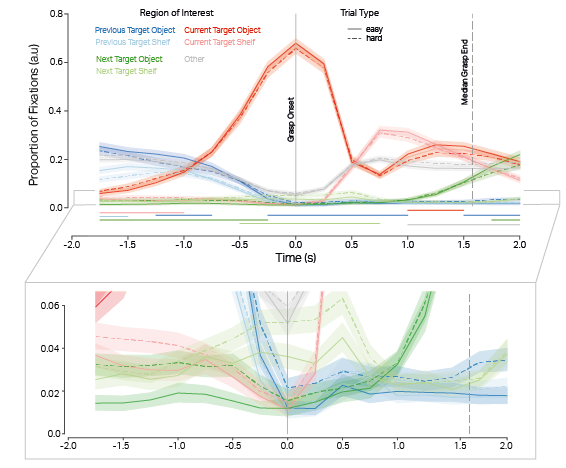
\includegraphics[width=1.\linewidth]{source/figures/results/results_22.png}
    \caption[Time course of fixations]{Proportion of fixations time-locked to the object displacement initiation (grasp onset) at time=0 and 2 seconds before and after on the seven regions of interest and for the EASY (solid trace) and HARD (dashed trace) tasks. In each time bin of 0.15s the proportion of fixations on all 7 ROIs for a trial type add up to 1. The dashed vertical line denotes the median end of the action execution phase The shaded regions show 95\% confidence interval of the mean proportion of gaze at each time-bin across all subjects. The proportion of fixations in each The horizontal traces at the bottom correspond to the significant time periods where the proportion of fixations on an ROI were different for the EASY and HARD trials.}
    \label{figure:action_locked}
\end{figure}


The proportion of fixations on the previous target object differed between EASY and HARD trials for three time periods. The first time period spanned from -1.25s to -0.75s (p-value<0.001) with lower proportion of fixations in the HARD tasks indicating allocation of gaze to other ROIs task-relevant to the action sequence. The second significant time period was from -0.25s to 1s (p-value<0.001) where the proportion of fixations were higher in the HARD tasks. This time period spans the start of the grasp onset till the execution of the object displacement strongly indicating that these fixations are related to monitoring of the execution of the current action and could be classified as 'checking' fixations. The third significant time period was from 1.5s to 2s (p-value<0.001) with higher proportion of fixations in the HARD trials. These differences might be constitutive of further 'checking' fixations in the case of HARD trials while executing the object displacement. 

The proportion of fixations on the previous target shelf were lower in the HARD trials compared to the EASY trials from -1.75s to -1.5s (p-value<0.001) before grasp onset. These differences suggest allocation of gaze to ROIs relevant to the task sequence happens earlier in the HARD tasks as more planning is required.

There were differences in the proportion of fixations on the current target object from 1s to 1.5s (p-value < 0.001) after grasp onset with lower proportion of fixations in the HARD tasks in this time period. These differences indicate that towards the end of action execution in HARD tasks fixations are allocated towards other task-relevant ROIs in the action sequence. Interestingly, there are no differences in the proportion of fixations on the current target object before the object displacement is initiated, suggesting that task complexity does not play a role in 'directing' fixations. 

There were higher proportion of fixations on the current target shelf in the HARD trials compared to EASY trials from -1.75s to -1s (p-value < 0.001) before grasp onset. These differences imply that some proportion of fixations are utilized to plan the current task, well before action has been initiated. These fixations could be classified as 'locating' fixations or look-ahead fixations which are predominantly present due to the complexity of the task. 

Similarly, there were a higher proportion of fixations on the next target object from -1.75s to -0.25s (p-value < 0.001) and a lower proportion from 1.75 s to 2s (p-value < 0.001). The differences in the first time period suggest that these fixations serve as 'locating' fixations to execute the next object displacement in the sequence. The presence of higher proportion of this fixations in the HARD tasks compared to EASY tasks indicates a need to plan the actions more thoroughly. The differences in the latter time period show a lower proportion of fixations for the HARD tasks indicating that prior locating fixations made it unnecessary to allocate attention to that object of interest. Conversely, in the EASY trials, the lower proportion of these locating fixations indicate an ad hoc gaze allocation for action execution.

There were also a higher proportion of fixations on the next target shelf from -0.5s to 0.75s (p-value < 0.001) in the HARD tasks. These fixations are made in concert with the onset of the action execution and indicate that these fixations are a play the role of both 'checking' fixations to monitor the task progression as well as 'locating' fixations to queue the locations in the scene that are important for the next action in the sequence.

Finally, the proportion of fixations on the other objects and shelves in the scene were higher in the HARD tasks from 1s to 2s (p-value < 0.001 ) after grasp onset. These differences indicate search behavior towards the end of the current task execution. Given the task complexity of the HARD trials, this search behavior might function to queue in further objects or shelves of interest in the subsequent action sequence. 


\begin{figure}[t]
    \centering
    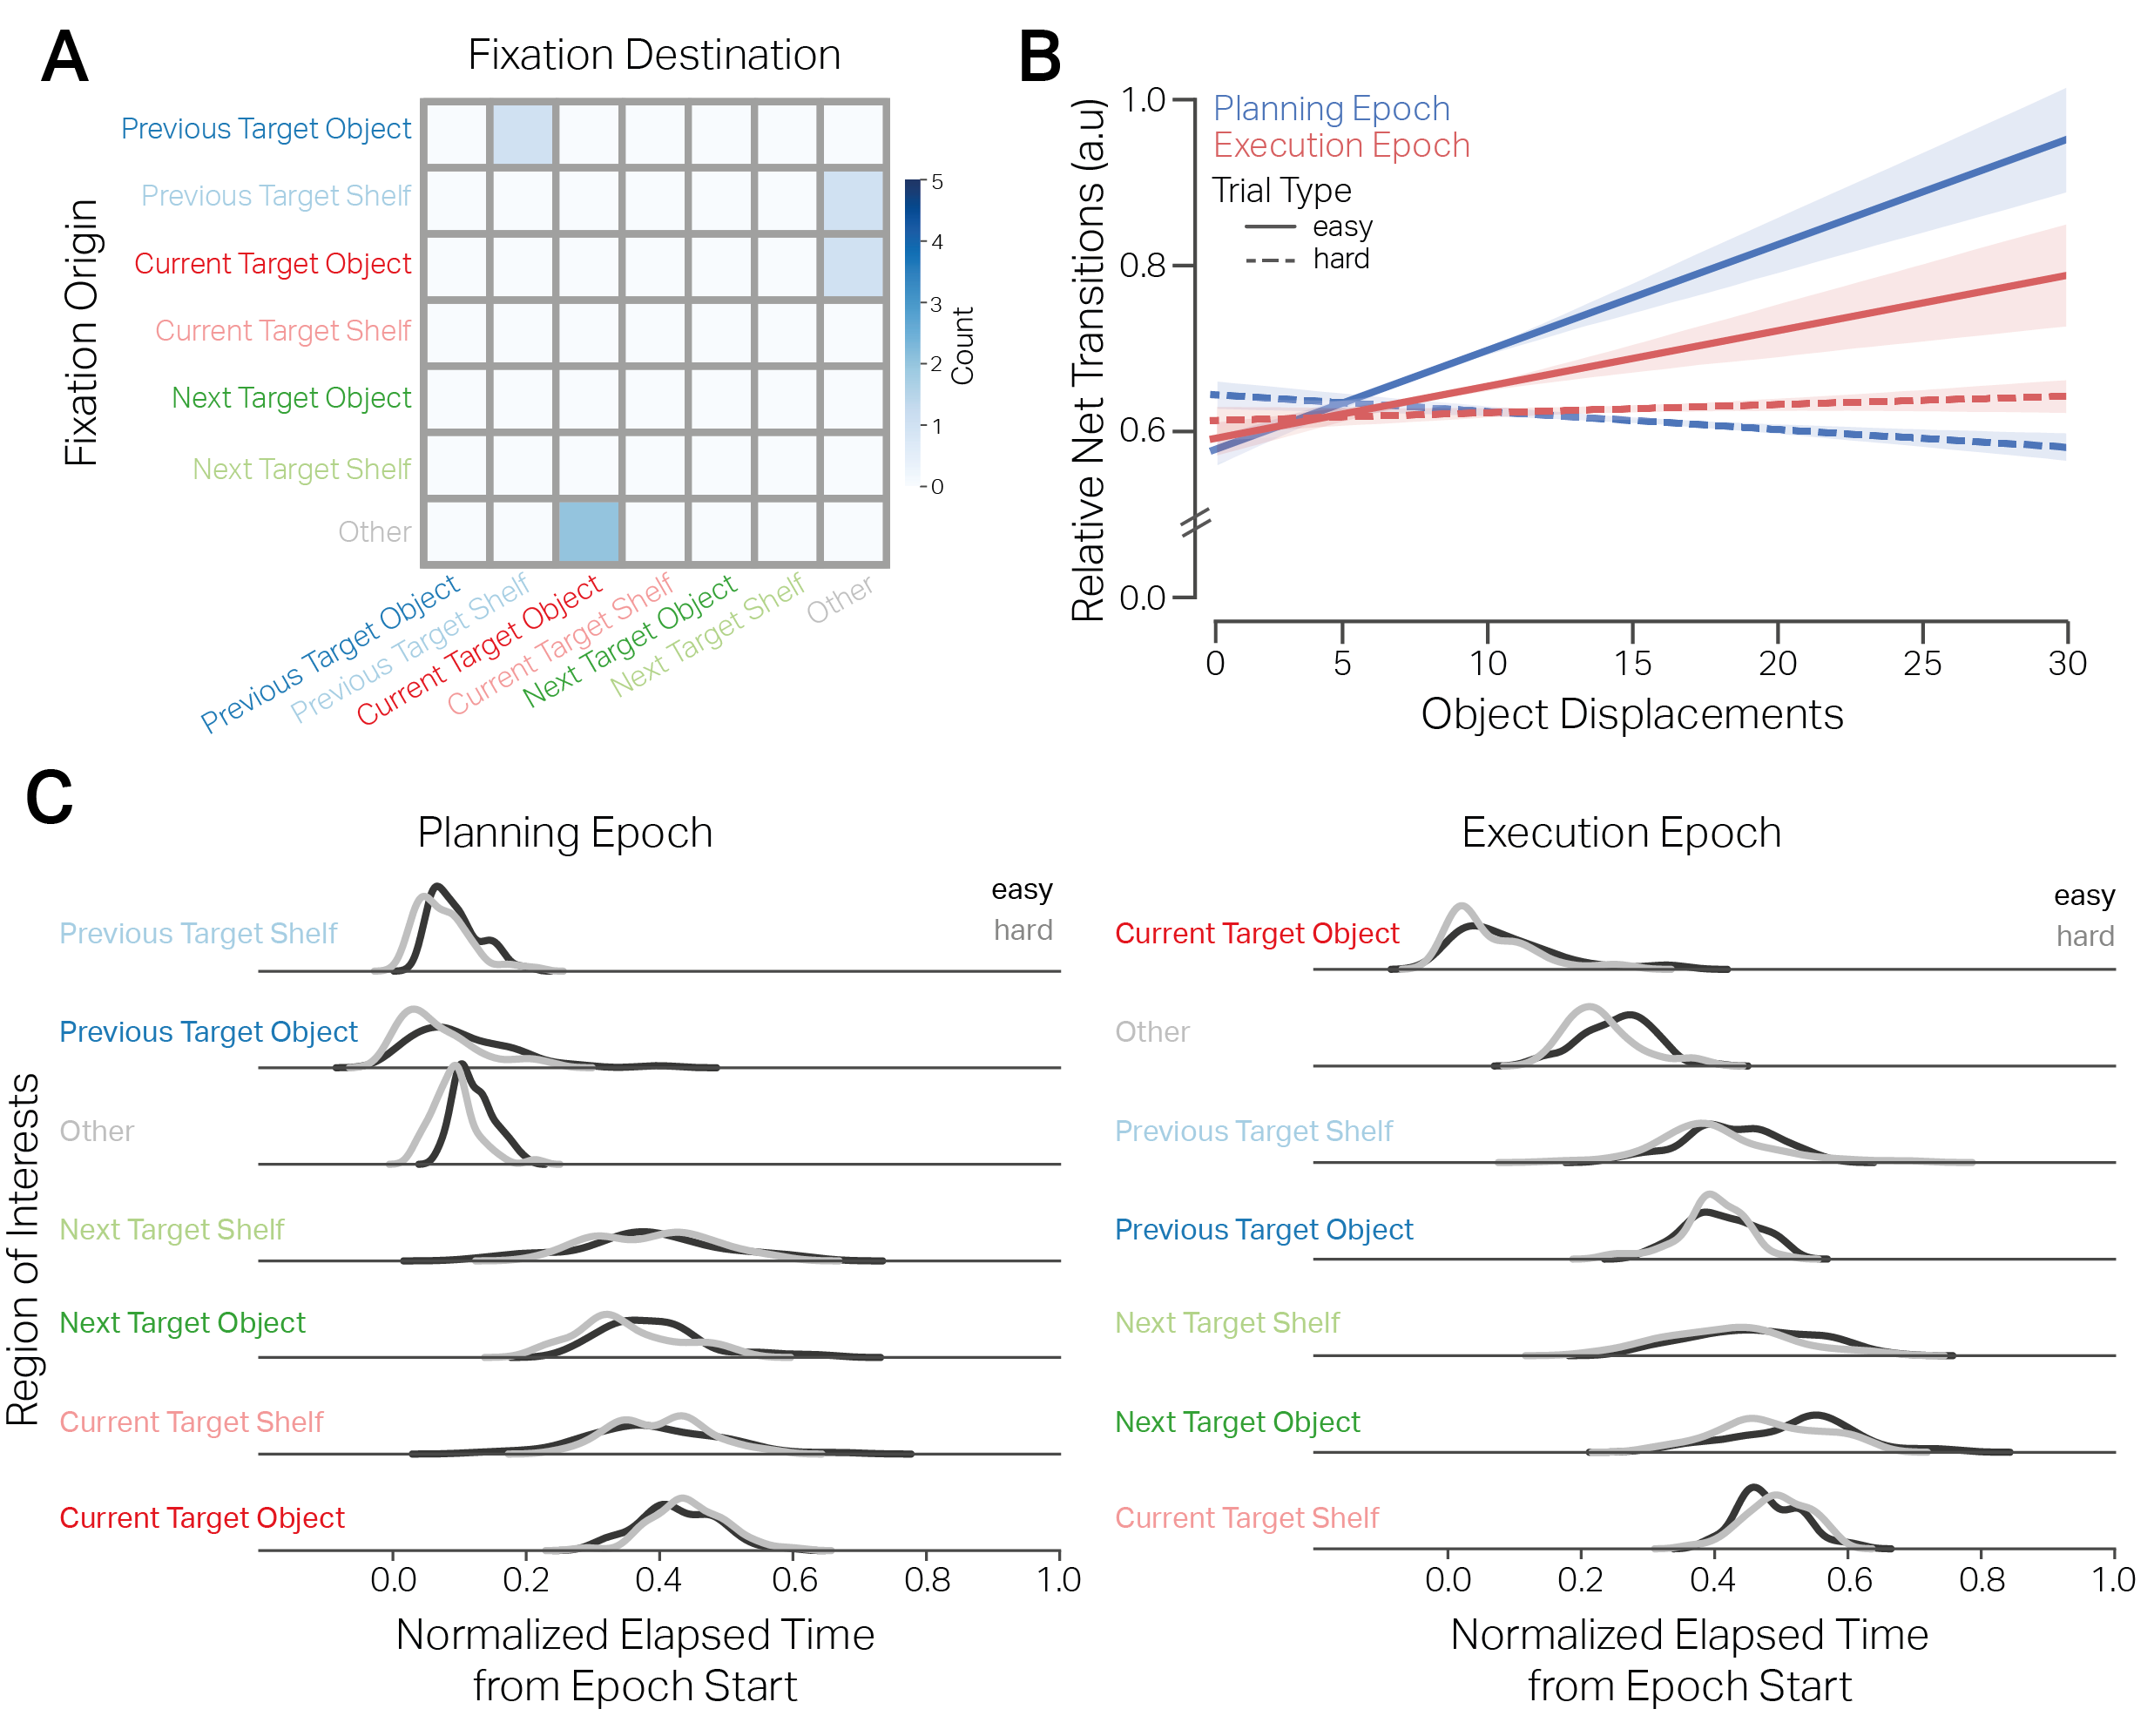
\includegraphics[width=1\linewidth]{source/figures/results/results_3.png}
    \caption[Spatiotemporal characteristics of gaze control]{\textbf{A.} Exemplar transition matrix for gaze switching in a planning epoch. The ordinate defines the origin of the gaze and the abscissa defines the destination of the gaze. \textbf{B.} Regression fit over the fixed-effects of trial types (EASY, HARD), epoch types (PLANNING, EXECUTION) and object displacements on the relative net transitions. The traces denote the the regression fit and the shaded region denotes 95\% confidence interval. \textbf{C.} Distributions of median time to first fixation on the 7 ROI for the action planning and execution epochs and trial types. The ordinate is sorted in ascending order of latency from epoch start for both planning and execution epochs. }
     \label{figure:spatiotemp}
\end{figure}


\subsection{Spatio-temporal Gaze Control in Action Planning and Execution}

The above results illustrate the average spatial and temporal aspects of attention during action planning and execution. However, the scanning behavior of subjects while they perform each action is "averaged out". In order to study the scanning behavior while subjects plan and execute an action, we computed transition matrices to capture fixations to and from each of the seven ROIs as described in Section \ref{sec:transitions}. \textcolor{Blue}{Figure \ref{figure:spatiotemp}A} shows the exemplar transition matrix for a planning epoch in an EASY trial. With the transition matrices we wanted to capture the gaze guidance behavior of the subjects while they plan and execute the actions. The relative net-transitions within the planning and execution epochs of a trial tell us the different functions of gaze guidance behaviors exhibited of the subjects. With higher relative net transitions, we expect higher gaze guidance to the current task-relevant ROIs, i.e, subjects perform saccades only for guiding their hand or body towards the current target object and less so for searching for task-relevant objects or monitoring the task. If subjects perform a search and fixate on multiple ROIs in an epoch, we would expect lower relative net transitions indicating a pattern of fixations related multiple task relevant schemas that compete for selection. 

In order to show the differences in mean gaze guidance behavior in a trial we used a linear mixed effects model (section \ref{sec:lmm}) with relative net transitions as the dependent variable and trial type (EASY, HARD), epoch type (PLANNING, EXECUTION) and number of object displacements as independent variables. As the independent variables were effect coded, the regression coefficients could be directly interpreted as main effects. \textcolor{Blue}{Figure \ref{figure:spatiotemp}B} illustrates the effects of trial type, epoch type and number of object displacements on the relative net transitions. There was a significant main effect of factor trial type (HARD - EASY) $\beta$ = -0.05 (95\%CI = [-0.06, -0.03], t(77.5)=-5.72), with a p-value < 0.001 showing that HARD trials had lower relative net transitions than EASY trials. There was also a significant main effect of factor epoch type (PLANNING - EXECUTION) $\beta$ = 0.03 (95\%CI = [0.00, 0.05], t(46.57)=-2.16), with a p-value = 0.03 showing that PLANNING epochs had higher relative net transitions than EXECUTION epochs. There was a significant effect of number of object displacements in a trial $\beta$ = 0.003 (95\%CI = [0.00, 0.01], t(57.64)=2.83), with a p-value = 0.006 showing that a one unit increase in the number of object displacements in a trial led to increase in relative net transitions by a factor of 0.003. There was a significant interaction between trial type and epoch type $\beta$ = -0.05 (95\%CI = [-0.08, -0.01], t(53.07)=-2.5), with a p-value = 0.01 showing that PLANNING epochs in HARD trials had lower relative net transitions. There was a significant interaction between trial type and number of object displacements $\beta$ = -0.009 (95\%CI = [-0.01, -0.01], t(45.82)=-4.31), with a p-value < 0.001 showing that a one unit increase in the number of object displacements in HARD trials led to increase in relative net transitions by a factor of -0.009. There was no significant interaction between epoch type and number of object displacements $\beta$ = 0.001 (95\%CI = [0.00, -0.01], t(43.20)=0.64), with a p-value = 0.52. There was a significant interaction between trial type, epoch type and number of object displacements $\beta$ = -0.01 (95\%CI = [-0.02, 0.00], t(42.67)=-2.20), with a p-value = 0.03 showing that a one unit increase in the number of object displacements in HARD trials and for PLANNING epochs led to increase in relative net transitions by a factor of -0.01.

The analysis above lends further evidence that task complexity had a significant effect on the gaze guidance behavior at the level of action planning and execution. The lower relative net transitions in the HARD tasks in general are indicative of competition between action schemas either for searching task-relevant ROIs or for monitoring the task progression. The higher relative net transitions in the EASY trials suggest saccades were primarily made towards the current task-relevant objects for directing or guiding the body or hand towards the object of interest. The significant correlation of the object displacements and the relative net transitions reveal that gaze allocation predominantly occurred in a just-in-time manner supporting the sub-optimal behavior exhibited by the subjects as well. 

To further disentangle the effect of task complexity on the order of gaze allocation to the task-relevant ROIs, we were interested in the latency of the first fixations to these . We used linear mixed effects regression to model the median time to first fixation on the 7 ROIs in each trial as described in section \ref{sec:lmm}. We modeled the latency of the first fixations for the planning and execution epochs separately. \textcolor{Blue}{Figure \ref{figure:spatiotemp}C} shows the distribution of the normalized time to first fixations on the seven ROIs for the action planning and execution epochs. 

In the action planning epoch, the time to first fixation on the previous target object was significantly earlier than the first fixation on the current target object $\beta$ = -0.35 (95\%CI = [-0.37, -0.32], t(49.67)=-29.01), with a p-value < 0.001. Similarly, the time to first fixation on the previous target shelf was significantly earlier than the first fixation on the current target object $\beta$ = -0.35 (95\%CI = [-0.37, -0.33], t(65.96)=-37.82), with a p-value < 0.001. The time to first fixation on other ROI was significantly earlier than the first fixation on the current target object $\beta$ = -0.33 (95\%CI = [-0.35, -0.31], t(72.37)=-37.03), with a p-value < 0.001. There was also a significant time difference between the first fixation on the next target object and the current target object $\beta$ = -0.06 (95\%CI = [-0.08, -0.05], t(47.36)=-6.96), with a p-value < 0.001. There was a significant time difference between the first fixation on the next target shelf and the current target object $\beta$ = -0.05 (95\%CI = [-0.07, -0.02], t(49.25)=-3.81), with a p-value < 0.001. Finally, there was also a significant time difference between the first fixation on the current target shelf and the current target object $\beta$ = -0.04 (95\%CI = [-0.06, -0.02], t(50.17)=-3.39), with a p-value = 0.001. When taking into account task complexity, there was a a significant interaction in the latency between previous target object and current target object $\beta$ = -0.06 (95\%CI = [-0.09, -0.02], t(123.78)=-3.11), with a p-value = 0.002. Similarly, there was also a significant interaction of trial type and time difference between first fixation between previous target shelf and current target object $\beta$ = -0.04 (95\%CI = [-0.07, -0.01], t(403.67)=-2.31), with a p-value = 0.02. There was also a significant interaction of trial type and latency between other ROI and current target object $\beta$ = -0.05 (95\%CI = [-0.08, -0.02], t(486.20)=-3.23), with a p-value = 0.001. There was also a significant interaction between trial type and latency between next target object and current target object $\beta$ = -0.05 (95\%CI = [-0.09, -0.02], t(83.82)=-3.16), with a p-value = 0.002. There was no significant interaction between trial type and the latency between next target shelf and current target object $\beta$ = -0.009 (95\%CI = [-0.05, 0.04], t(52.01)=-0.39), with a p-value = 0.69. There was also no significant interaction between trial type and delay between current target shelf and current target object $\beta$ = -0.002 (95\%CI = [-0.04, 0.04], t(55.39)=-0.10), with a p-value = 0.91.

Taken together, the irrespective of task complexity, the action planning epochs show a systematic progression of fixations from one ROI to another. This structured temporal sequence of fixations with a defined temporal window shows that the look-ahead fixations pertaining to the future action relevant ROIs are not incidental and part of the cognitive schema to accomplish the task. Moreover, given the task complexity, the temporal profiles of these look-ahead fixations can change and occur slightly earlier.

In the action execution epoch, the time to first fixation on the other ROI was significantly later than the first fixation on the current target object $\beta$ = 0.17 (95\%CI = [0.14, 0.19], t(50.47)=11.40), with a p-value < 0.001. Similarly, the time to first fixation on the previous target object was significantly later than the first fixation on the current target object $\beta$ = 0.033 (95\%CI = [0.30, 0.35], t(61.73)=24.57), with a p-value < 0.001. The time to first fixation on previous target shelf was also significantly later than the first fixation on the current target object $\beta$ = 0.33 (95\%CI = [0.30, 0.36], t(52.69)=23.59), with a p-value < 0.001. There was a significant time difference between the first fixation on the next target object and the current target object $\beta$ = 0.36 (95\%CI = [0.33, 0.39], t(58.75)=24.56), with a p-value < 0.001. There was a significant time difference between the first fixation on the next target shelf and the current target object $\beta$ = 0.43 (95\%CI = [0.40, 0.46], t(54.68)=28.49), with a p-value < 0.001. Finally, there was also a significant time difference between the first fixation on the current target shelf and the current target object $\beta$ = 0.42 (95\%CI = [0.39, 0.44], t(64.75)=32.13), with a p-value < 0.001. When taking into account task complexity, there was no significant interaction in the latency between other ROI and current target object $\beta$ = 0.008 (95\%CI = [-0.03, 0.05], t(136.42)=0.40), with a p-value = 0.69. There was no significant interaction between trial type and latency between previous target object and current target object $\beta$ = 0.02 (95\%CI = [-0.02, 0.07], t(116.24)=0.96), with a p-value = 0.34. There was no significant interaction between trial type and the latency between previous target shelf and current target object $\beta$ = 0.01 (95\%CI = [-0.04, 0.05], t(98.32)=0.49), with a p-value = 0.62.There was no significant interaction of trial type and time difference between first fixation between next target object and current target object $\beta$ = -0.002 (95\%CI = [-0.06, 0.05], t(60.67)=-0.10), with a p-value = 0.92. There was also no significant interaction of trial type and latency between next target shelf and current target object $\beta$ = -0.01 (95\%CI = [-0.07, 0.05], t(63.53)=-0.35), with a p-value = 0.73. There was a significant interaction between trial type and delay between current target shelf and current target object $\beta$ = 0.05 (95\%CI = [0.00, 0.09], t(122.10)=2.15), with a p-value = 0.03.

In sum, irrespective of the task complexity, the action execution epochs show a systematic sequence of first fixations on the seven ROIs. The fixations on the previous action related object and shelf show that a monitoring of the current action with respect to the previous action might be at play, where these fixations are made to confirm the choice of the current target shelf and might serve as look-back fixations. Similarly, fixations on the target object and shelf for the next action might serve as look-ahead fixations. However, with increasing task complexity, the temporal sequence of the first fixations remained unchanged except for the later gaze allocation to the current target shelf in the case of HARD trials. One may posit here that the added task complexity does not affect the temporal sequence of the gaze allocation during action execution.